%%%%%%%%%%%%%%%%%%%% Document code starts here %%%%%%%%%%%%%%%%%%%%
\subsubsection{Alcance}
Esta parte de ISO / IEC 14443 especifica un protocolo de transmisión de bloques semidúplex que presenta las necesidades especiales de un entorno sin contacto y define la secuencia de activación y desactivación del protocolo.\par

Esta parte de ISO / IEC 14443 se utilizará junto con otras partes de ISO / IEC 14443 y se aplica a las tarjetas de proximidad de tipo A y tipo B.\par

\subsubsection{Referencias normativas}
Las siguientes normas contienen disposiciones que, a través de la referencia en este texto, constituyen disposiciones de esta parte de ISO / IEC 14443. En el momento de la publicación, las ediciones indicadas eran válidas. Todos los estándares están sujetos a revisión,\par

y se alienta a las partes de los acuerdos basados ​​en esta parte de ISO / IEC 14443 a investigar la posibilidad de aplicar las normas Internacionales válidas más recientes.\par

ISO / IEC 7816-3, Tarjetas de identificación - Tarjetas de circuito (s) integrado (s) con contactos - Parte 3: señales electrónicas y protocolos de transmisión.\par

ISO / IEC 7816-4, Tarjetas de identificación - Tarjetas de circuito (s) integrado (s) con contactos - Parte 4: Comandos interindustriales para el intercambio.\par

\subsubsection{Término (s) y definición (es)}
\paragraph{Duración del bit.}
La duración del bit se define como una unidad de tiempo elemental (ETU). El ETU se calcula con la siguiente fórmula:\par

1 etu = 128 / (D x fc)\par

El valor inicial del divisor D será 1.\par

La frecuencia portadora fc se define en ISO / IEC 14443-2.\par

\paragraph{Bloque.}
Un tipo especial de trama, que contiene un formato de datos de protocolo válido. Un formato de datos de protocolo válido incluye I-blocks, R-blocks o S-blocks.\par

\paragraph{Bloque inválido.}
Un tipo de trama, que contiene un formato de protocolo no válido. Un tiempo de espera, cuando no se ha recibido ningún marco, no es interpretado como un bloque inválido.\par

\paragraph{Trama}
Como se define en ISO / IEC 14443-3. El PICC tipo A usa la trama estándar definido para el tipo A y el PICC tipo B usa la trama definido para el tipo B.\par


\vspace{\baselineskip}
\subsubsection{Símbolos (y términos abreviados)}
\begin{itemize}
	\item ACK - Reconocimiento positivo\par

	\item ATS - Respuesta a SELECT\par

	\item ATQB - Respuesta a la búsqueda de PICC tipo B\par

	\item CID - IDentificador de tarjeta\par

	\item CRC - Comprobación de redundancia cíclica, como se define para cada tipo de PICC en ISO / IEC 14443-3\par

	\item D - Divisor\par

	\item DR - Divisor recibido (PCD a PICC)\par

	\item DS - Divisor enviado (PICC a PCD)\par

	\item EDC - Código de detección de errores\par

	\item ETU - Unidad de tiempo elemental\par

	\item fc - Frecuencia portadora\par

	\item FSC - Tamaño de la trama para la tarjeta de proximidad\par

	\item FSD - Tamaño de la trama para el dispositivo de acoplamiento de proximidad\par

	\item FWT - Tiempo de espera de tramas\par

	\item FWTTEMP - Tiempo de espera temporal de trama\par

	\item HLTA - Comando HALT para PICC tipo A\par

	\item I-block - Bloque de información\par

	\item INF - Campo de información\par

	\item NAD - Nodo de dirección\par

	\item NAK - No reconocido\par

	\item OSI - Interconexión de sistemas abiertos\par

	\item PCB -Byte de control de protocolo\par

	\item PCD - Dispositivo de acoplamiento de proximidad\par

	\item PICC - Tarjeta de proximidad\par

	\item PPS - Protocolo y selección de parámetros\par

	\item PPSS - Inicio de protocolos y selección de parámetros\par

	\item PPS0 - Protocolo y selección de parámetros 0\par

	\item PPS1 - Protocolo y selección de parámetros 1\par

	\item R-block - Bloque READY recibido\par

	\item R (ACK) - R-block que contiene un reconocimiento positivo\par

	\item R (NAK) - R-block que contiene un reconocimiento negativo\par

	\item RATS - Solicitud de respuesta para SELECT\par

	\item RFU - Reservado para uso futuro\par

	\item S-block - Bloque de supervisión\par

	\item SAK - Reconocimiento de SELECT\par

	\item SFGT - Tiempo de protección de inicio de trama\par

	\item WUPA - Comando Wake-Up para PICC tipo A\par

	\item WTX - Extensión del tiempo de espera\par

	\item WTXM - Multiplicador de la extensión de tiempo de espera
\end{itemize}\par

\paragraph{Activación de protocolo de PICC tipo A}
Se aplicará la siguiente secuencia de activación: \par

\begin{itemize}
	\item Secuencia de activación de PICC como se define en ISO / IEC 14443-3 (petición, ciclo anticolisión y selección).\par

	\item Al principio, se debe verificar el byte SAK para determinar la disponibilidad de un ATS. El SAK se define en ISO / IEC 14443-3.\par

	\item El PICC puede configurarse en estado HALT, usando el comando HLTA como se define en ISO / IEC 14443-3, si no hay ATS disponible.\par

	\item El PCD puede enviar el RATS como siguiente comando después de recibir el SAK si hay un ATS disponible.\par

	\item El PICC enviará su ATS como respuesta a las RATS. El PICC solo responderá a las RATS si la RATS es recibido directamente después de la selección.\par

	\item Si el PICC admite cualquier parámetro modificable en el ATS, el PCD puede utilizar una solicitud de PPS como siguiente comando después de recibir el ATS para cambiar los parámetros.\par

	\item El PICC enviará una respuesta de PPS como respuesta a la solicitud de PPS.
\end{itemize}\par

Un PICC no necesita implementar el PPS, si no admite ningún parámetro modificable en el ATS.\par



%%%%%%%%%%%%%%%%%%%% Figure/Image No: 1 starts here %%%%%%%%%%%%%%%%%%%%

\begin{figure}[H]
	\begin{center}
		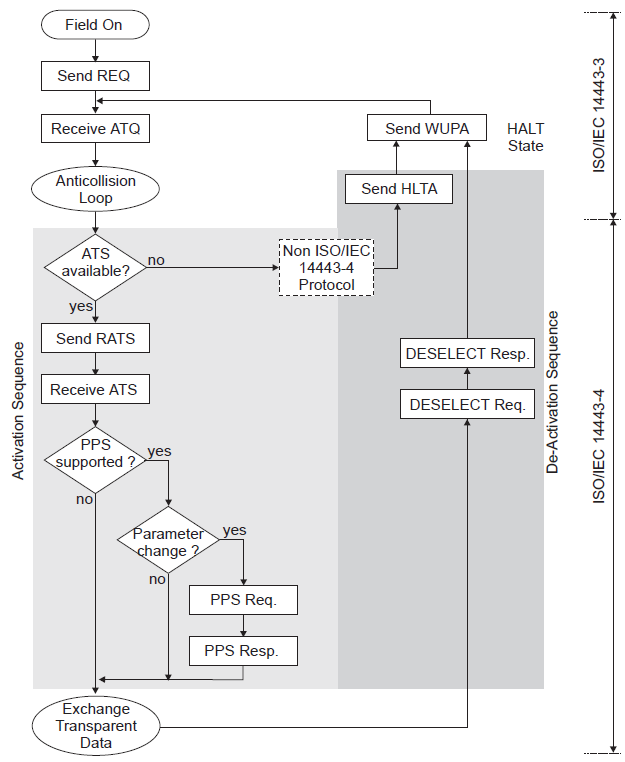
\includegraphics[width=6.27in,height=7.64in]{Norma_ISO/14443-4/media/image8.png}
    \end{center}
\end{figure}


%%%%%%%%%%%%%%%%%%%% Figure/Image No: 1 Ends here %%%%%%%%%%%%%%%%%%%%

\par
\begin{center}
\textbf{Figura 3.8.5.1 - Activación de un PICC Tipo A desde un PCD}
\end{center}
\par

\paragraph{Solicitud de respuesta para seleccionar}
Esta cláusula define las RATS con todos sus campos\par

El byte de parámetro consta de dos partes (figura 3.8.5.2):\par

El medio byte b8 a b5 más significativo se denomina FSDI y codifica FSD. El FSD define el tamaño máximo de una trama que el PCD puede recibir.\par

El medio byte menos significativo b4 a b1 se denomina CID y define el número lógico del PICC direccionado en el rango de 0 a 14. El valor 15 es RFU. El CID está especificado por el PCD y será único para todos PICCs, que están en el estado ACTIVO al mismo tiempo. El CID se fija por el tiempo que el PICC está activo y el PICC usará el CID como su identificador lógico, que está contenido en el primer RATS sin errores recibido.\par


\vspace{\baselineskip}


%%%%%%%%%%%%%%%%%%%% Figure/Image No: 2 starts here %%%%%%%%%%%%%%%%%%%%

\begin{figure}[H]
	\begin{center}
		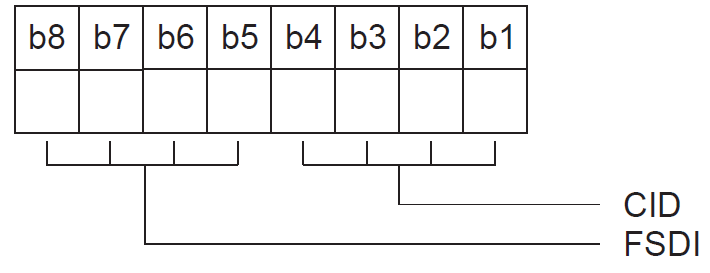
\includegraphics[width=3.84in,height=1.48in]{Norma_ISO/14443-4/media/image5.png}
    \end{center}
\end{figure}


%%%%%%%%%%%%%%%%%%%% Figure/Image No: 2 Ends here %%%%%%%%%%%%%%%%%%%%

\par
\begin{center}
\textbf{Figura 3.8.5.2 - Byte de parámetros del comando RATS.}
\end{center}
\par

\paragraph{Respuesta a SELECT}
Esta cláusula define el ATS con todos sus campos disponibles (Figura 3.8.5.3).\par

En el caso de que uno de los campos definidos no esté presente en un ATS enviado por un PICC, se aplicarán los valores predeterminados para ese campo.\par


\vspace{\baselineskip}


%%%%%%%%%%%%%%%%%%%% Figure/Image No: 3 starts here %%%%%%%%%%%%%%%%%%%%

\begin{figure}[H]
	\begin{center}
		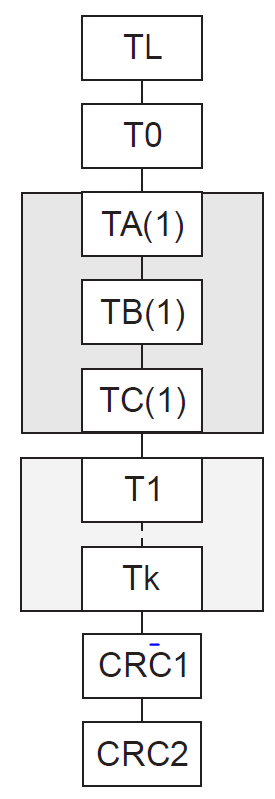
\includegraphics[width=0.88in,height=2.56in]{Norma_ISO/14443-4/media/image3.png}
    \end{center}
\end{figure}


%%%%%%%%%%%%%%%%%%%% Figure/Image No: 3 Ends here %%%%%%%%%%%%%%%%%%%%

\par

\begin{center}
\textbf{Figura 3.8.5.3 - Estructura del comando ATS.}
\end{center}
\par

\paragraph{Estructura de los bytes}
El byte de longitud TL viene seguido de un número variable de bytes posteriores opcionales en el siguiente orden:\par

\begin{itemize}
	\item formato de bytes T0,\par

	\item bytes de interfaz TA (1), TB (1), TC (1) y bytes históricos T1 a Tk.
\end{itemize}\par

\paragraph{Longitud de bytes}
El TL de longitud de bytes es obligatorio y especifica la longitud del ATS transmitido incluido él mismo. Los dos bytes CRC no están incluidos en TL. El tamaño máximo del ATS no debe exceder el FSD indicado. Por lo tanto, el valor máximo de TL no debe exceder el FSD-2.\par

\paragraph{Formato de byte}
El byte de formato T0 es opcional y está presente tan pronto como la longitud sea mayor que 1. El ATS solo puede contener los siguientes bytes opcionales, cuando este byte de formato está presente.\par

T0 consta de tres partes:\par

\begin{itemize}
	\item El bit más significativo b8 se establecerá en 0. El valor 1 es RFU.\par

	\item Los bits b7 a b5 indican la presencia de bytes de interfaz posteriores TA (1), TB (1) y TC (1).\par

	\item El medio byte menos significativo b4 a b1 se llama FSCI y codifica FSC. El FSC define el tamaño máximo de un marco aceptado por el PICC. El valor predeterminado de FSCI es 2 y conduce a un FSC de 32 bytes. La codificación de FSC es igual a la codificación de FSD.
\end{itemize}\par

\paragraph{Byte de interfaz TA (1)}
El byte de interfaz TA (1) consta de cuatro partes:\par

\begin{itemize}
	\item El bit más significativo b8 codifica la posibilidad de manejar diferentes divisores para cada dirección. Cuando este bit se establece en 1, el PICC no puede manejar diferentes divisores para cada dirección.\par

	\item Los bits b7 a b5 codifican la capacidad de tasa de bits del PICC para la dirección de PICC a PCD, llamada DS. El valor predeterminado será (000) b.\par

	\item El bit b4 se establece en (0) b y el otro valor es RFU.\par

	\item Los bits b3 a b1 codifican la capacidad de velocidad de bits del PICC para la dirección de PCD a PICC, llamada DR. El valor predeterminado será (000) b.
\end{itemize}\par

\paragraph{Byte de interfaz TB (1)}
El\ byte de interfaz TB (1) transmite información para definir el tiempo de espera de la trama y el tiempo de guarda  de la trama de inicio.\par

El byte de interfaz TB (1) consta de dos partes:\par

\begin{itemize}
	\item El medio byte b8 a b5 más significativo se denomina FWI y codifica FWT\par

	\item El medio byte menos significativo b4 a b1 se llama SFGI y codifica un valor multiplicador utilizado para definir el SFGT. El SFGT define un tiempo de protección específico que necesita el PICC antes de estar listo para recibir el siguiente cuadro después de haber enviado el ATS. SFG está codificado en el rango de 0 a 14. El valor de 15 es RFU. El valor de 0 indica que no se necesita SFGT y los valores en el rango de 1 a 14 se usan para calcular el SFGT con la fórmula que se indica a continuación. El valor predeterminado de SFG es 0.
\end{itemize}\par

\begin{center}
 \( SFGT= \left( 256\ast\frac{16}{fc} \right) \ast2^{SFG} \) 
\end{center}
\par

\paragraph{Bytes históricos}
Los bytes históricos T1 a Tk son opcionales y aportan información general. La longitud máxima de ATS da la cantidad máxima posible de bytes históricos. ISO / IEC 7816-4 especifica el contenido de los bytes históricos.\par

\paragraph{Petición de selección de protocolo y parámetro}
La solicitud de PPS contiene el byte de inicio seguido de un byte de formato y un byte de parámetro (figura 3.8.5.4).\par


\vspace{\baselineskip}


%%%%%%%%%%%%%%%%%%%% Figure/Image No: 4 starts here %%%%%%%%%%%%%%%%%%%%

\begin{figure}[H]
	\begin{center}
		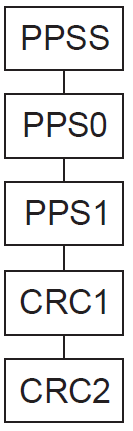
\includegraphics[width=0.53in,height=1.7in]{Norma_ISO/14443-4/media/image7.png}
    \end{center}
\end{figure}


%%%%%%%%%%%%%%%%%%%% Figure/Image No: 4 Ends here %%%%%%%%%%%%%%%%%%%%

\par
\begin{center}
\textbf{Figura 3.8.5.4 - Solicitud de selección de protocolo y parametros.}
\end{center}
\par

\paragraph{Inicio de selección de protocolo y parámetros}
El PPSS consta de dos partes:\par

\begin{itemize}
	\item El medio byte más significativo b8 a b5 es igual a 'D' e identifica el PPS.\par

	\item El medio byte menos significativo b4 a b1 se denomina CID y define el número lógico del PICC direccionado.
\end{itemize}\par

\paragraph{Selección 0 de protocolo y parámetros.}
El PPS0 consta de cuatro partes:\par

\begin{itemize}
	\item b8 a b6 deberá establecerse en (000)b, todos los demás valores son RFU\par

	\item b5 si el PPS1 es transmitido se establece en (1)b.\par

	\item b4 a b2 deberá establecerse en (000)b, todos los demás valores son RFU\par

	\item b1deberá establecerse en (1)b, (0)b es RFU
\end{itemize}\par

\paragraph{Selección 1 de protocolo y parámetros.}
El PPS1 consta de tres partes:\par

\begin{itemize}
	\item El medio byte más significativo b8 a b5 es (0000) b y todos los demás valores son RFU.\par

	\item Los bits b4, b3 se llaman DSI y codifican el divisor entero seleccionado de PICC a PCD.\par

	\item Los bits b2, b1 se llaman DRI y codifican el divisor entero seleccionado de PCD a PICC.
\end{itemize}\par

\paragraph{Respuesta de selección de protocolo y parámetros}
La respuesta de PPS confirma la solicitud de PPS recibida.\par

\paragraph{Tiempo de espera de la trama de activación}
El tiempo de espera de la trama de activación define el tiempo máximo para que un PICC comience a enviar su trama de respuesta después del final de una trama recibida del PCD y tiene un valor de 65536 / fc ($ \sim $  4833 $ \mu $ s).\par

\paragraph{Detección y recuperación de errores}
\paragraph{Manejo de RATS y ATS}
\paragraph{Reglas de PCD}
Cuando el PCD ha enviado el RATS y recibe un ATS válido, el PCD continuará funcionando.\par

En cualquier otro caso, el PCD puede retransmitir la RATS antes de que utilice la secuencia de desactivación tal como se define en la cláusula 8.\par

\paragraph{Reglas del PICC}
Cuando el PICC ha sido seleccionado con el último comando y\par

\begin{enumerate}
	\item Recibe un RATS válido, el PICC deberá\par

\begin{itemize}
	\item enviar de vuelta su ATS y\par

	\item deshabilitar las RATAS (no responda más a las RATS recibidas).
\end{itemize}\par

	\item Recibe cualquier otro bloque válido o inválido, excepto un comando HLTA, el PICC deberá
\end{enumerate}\par

\begin{itemize}
	\item ignorar el bloque y permanezca en modo de recepción.
\end{itemize}\par

\paragraph{Tratamiento de solicitud PPS y respuesta PPS}
\paragraph{Reglas del PCD}
Cuando el PCD ha enviado una solicitud de PPS y recibió una respuesta de PPS válida, el PCD activará los parámetros seleccionados y continuará la operación.\par

En cualquier otro caso, el PCD puede retransmitir una solicitud de PPS y continuar la operación.\par

\paragraph{Reglas de PICC }
Cuando el PICC ha recibido un RATS, envía su ATS y\par

\begin{enumerate}
	\item 1. recibió una solicitud de PPS válida, el PICC deberá\par

\begin{itemize}
	\item envía la respuesta de PPS,\par

	\item deshabilitar la solicitud de PPS (ya no responde a las solicitudes de PPS recibidas) y\par

	\item activar el parámetro recibido.
\end{itemize}\par

	\item Recibió un bloque inválido, el PICC deberá\par

\begin{itemize}
	\item deshabilitar la solicitud de PPS (ya no responde a las solicitudes de PPS recibidas) y\par

	\item permanecer en modo de recepción.
\end{itemize}\par

	\item Recibió un bloque válido, excepto una solicitud de PPS, el PICC deberá
\end{enumerate}\par

\begin{itemize}
	\item deshabilitar la solicitud de PPS (ya no responde a las solicitudes de PPS recibidas) ycontinuar operando
\end{itemize}\par

\paragraph{Manejo del CID durante la activación}
Cuando el PCD ha enviado un RATS que contiene un CID = n distinto a 0 y\par

\begin{enumerate}
	\item Recibió un ATS que indica que el CID es compatible, el PCD deberá\par

\begin{itemize}
	\item enviar bloques que contengan CID = n a este PICC\par

	\item no usar el CID = n para RATS adicionales mientras este PICC esté en estado ACTIVE.
\end{itemize}\par

	\item Recibió un ATS que indica que el CID no es compatible, el PCD deberá enviar bloques que no contengan CID a este PICC y no activar ningún otro PICC mientras este PICC esté en estado ACTIVE.
\end{enumerate}\par

Cuando el PCD ha enviado un RATS que contiene un CID igual a 0 y\par

\begin{enumerate}
	\item Recibió un ATS que indica que CID es compatible, el PCD puede\par

\begin{itemize}
	\item enviar bloques que contengan CID igual a 0 a este PICC\par

	\item no activar ningún otro PICC mientras este PICC esté en estado ACTIVE.
\end{itemize}\par

	\item Recibió un ATS que indica que el CID no es compatible, el PCD deberá
\end{enumerate}\par

\begin{itemize}
	\item enviar bloques que no contengan CID a este PICC y no activar ningún otro PICC mientras este PICC esté en estado ACTIVE.
\end{itemize}\par